



\section{Additional Results in Model Wind Tunnel Experiments}

\subsection{$\mu$P hyper-parameter search}
\label{app:bayesiansearch}
We conduct an extensive Bayesian search over a set of predefined parametric spaces. For efficiency, we search for the $N=0.009B$ model. In our pilot experiments, we confirm that when hyper-parameter optimization is conducted using datasets scaled at magnitudes of 10N and 20N, there is a consistency observed in the efficacy of hyper-parameters. Therefore, we train the models with $|D| = 10N = 0.09B$ tokens.
Meanwhile, we also try QK-Norm~\citep{henry-etal-2020-query} and independent weight decay~\citep{loshchilov2017decoupled} as well to stabilize the learning rate. The overall results are shown in Figure~\ref{fig:mupsearch_app}. After applying the QK-norm, we observe a significant decrease in the learning rate sensitivity similar to~\cite{wortsman2023small}. However, as the MiniCPM project itself is an SLM, we do not require low learning rate sensitivity as long as we find the best learning rate with TensorProgram~\citep{yang2022tensor, yang2023tensor}. Therefore, we do not introduce QK-norm and independent weight decay in later experiments of MiniCPM. In Figure~\ref{fig:mupsearch_app}, we identify the best hyper-parameters for $scale\_depth=1.4$, $scale\_emb=12$, $init\_std=0.1$, and $lr=0.01$. 


\begin{figure}[htbp]
    \centering
    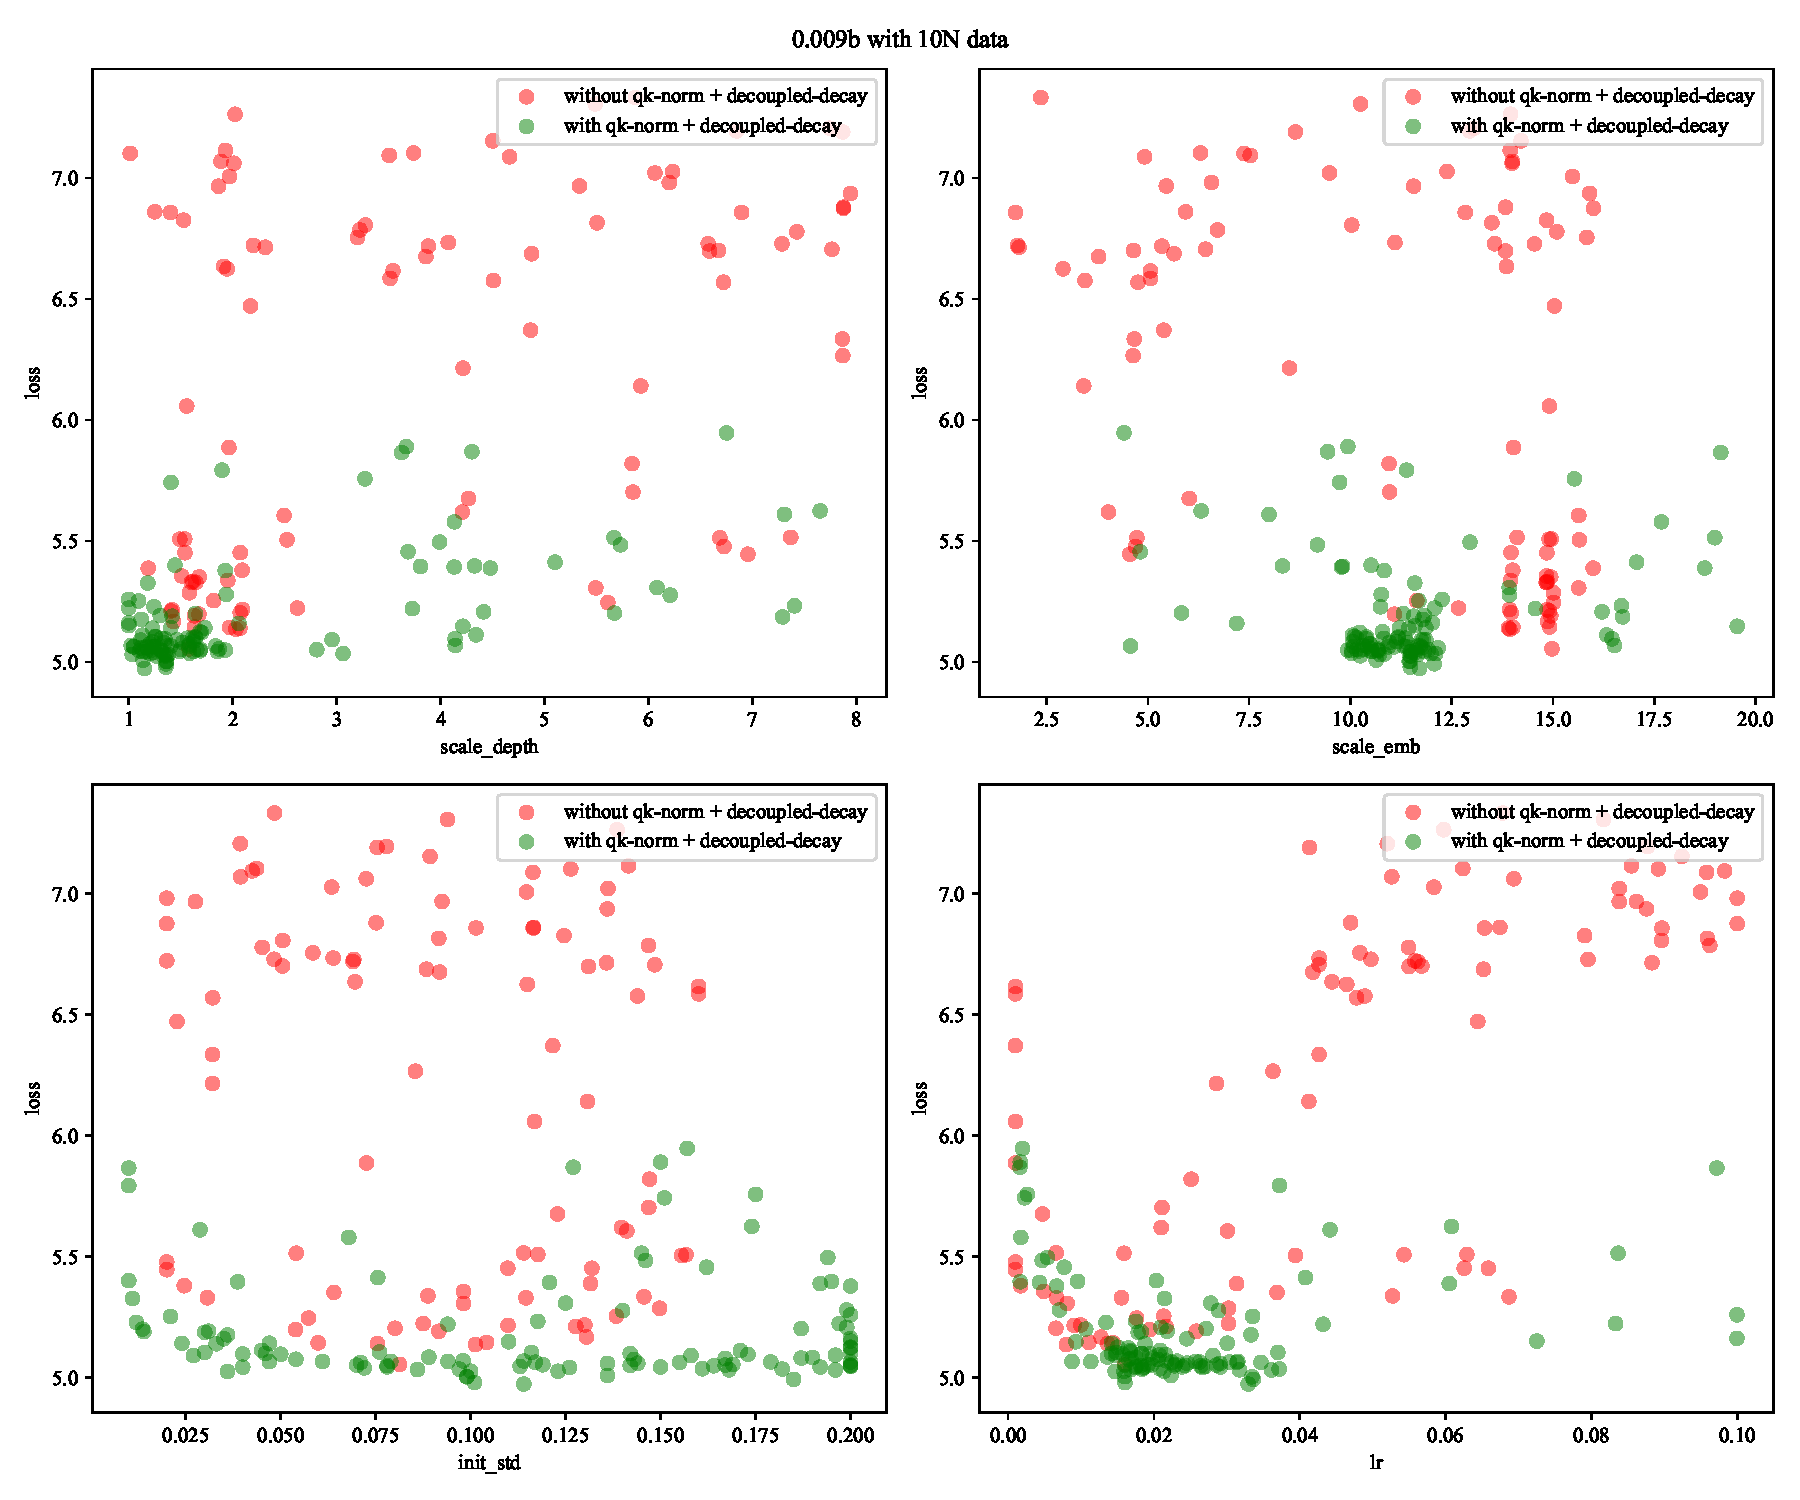
\includegraphics[width=0.65\linewidth]{Fig/mup0.009bwith10Ndata.pdf}
    \caption{Grid search over the $\mu$P parameterization spaces.}
    \label{fig:mupsearch_app}
\end{figure}


\begin{table}[h]
\centering
\begin{tabular}{l|p{8cm}}
\toprule
\textbf{Name}                       & \textbf{Specific Operation}                                                                                                                 \\ \midrule
Embedding Output Scaling            & Multiply the output of the embedding by $scale\_{emb}$                                                                                                                                                     \\ \hline
Residual Connection Scaling         & Scale the output tensor of a block before adding to each residual connection in each layer by $scale\_{depth}/\sqrt{\text{num\_layers}}$ 
\\ \hline
Initialization of Tensors           & Set the initialization standard deviation of each two-dimensional tensor parameter to $init\_std/\sqrt{d_m/d_{base}}$, and set other parameters' initialization to 0.1                  \\ \hline
Learning Rate Scaling of Tensors    & Adjust the learning rate of each two-dimensional tensor parameter to $1/({d_m/d_{base}}) $ times the learning rate of other parts (or the overall learning rate)                    \\ \hline
LM Head Scaling                    & Adjust the output logits to $1/(d_m/d_{base})$ times the original value                                                                                                           \\ \bottomrule
\end{tabular}
\caption{List of operations used when applying tensor program techniques.}
\label{tab:mup}
\end{table}

\subsection{Comment on Optimal Batchsize}
\label{app:batchsize}
In~\cite{kaplan2020scaling}, OpenAI studies the relationship between the loss function and the number of tokens. In their experiments, they assume that consuming more steps is equivalent to consuming more time. Under this assumption, OpenAI defines a critical batch size that achieves a certain loss without consuming too many steps or tokens. This rationale is valid if the experiments are provided with unlimited GPUs (at least within the scope of the experiments). Since GPUs are unlimited, enlarging batch size will not increase the single-step duration but will decrease the total number of steps. However, in our experiment, since we have a fixed resource (number of GPUs), we observe that doubling the batch size almost equals doubling the single-step time. Therefore, enlarging batch size to decrease total training steps has minimal effect on the total training time. In light of this observation, we drop the goal of ``not consuming too many steps'' and turn towards minimizing the token quantity to achieve the lowest loss, instead.

The observation regarding the estimation of optimal batch size in relation to loss resembles the "Chicken-and-egg" paradox. Practically, there's often a preliminary estimate of the achievable loss for a given model size, informed by prior knowledge of preliminary experiments. However, there is potential for the development of more refined estimation procedures in the future.

The optimal batch size and optimal learning rate are likely to be not independent. To overcome this correlation, we do a preliminary study on the learning rate first, then choose an optimal learning rate to do a batch size experiment, and use batch size scaling to do the learning rate again. This is a bit like the Coordinate Descent optimization method. However, more rigorous methods are welcomed in future work.


\subsection{Model Architecture in Model Wind Tunnel Experiments}
We list the model configuration used in the model wind tunnel experiments in Table~\ref{tab:appmodel_configs}. The ``shape'' of the model, i.e., model width compared to model depth is kept as similar as possible to avoid any potential performance variation.

\begin{table}[htbp]
    \centering
    \begin{tabular}{c|cccccc}
    \toprule
        \textbf{Name} & \textbf{N (B)}& $d_m$ & $d_{ff}$ &$d_h$ & $n_h$ & $L$ \\
    \midrule
          9M    &  0.009 & 320 & 800 & 64 & 5 & 8\\
           30M &   0.036 & 512 & 1280 & 64 & 8 & 12  \\
          70M &  0.066 & 640 & 1600 & 64 & 10 & 14\\
          0.1B &  0.109 & 768 & 1920 & 64 & 12 & 16  \\
         0.17B &  0.166 & 896 & 2240 & 64 & 14 & 18 \\
         0.2B&  0.241 & 1024 & 2560 & 64 & 16 & 20 \\
        0.5B& 0.499 & 1344 & 3360 & 64 & 21 & 24 \\
    \bottomrule
    \end{tabular}
    \caption{Model configurations and training configurations of the models in the scaling curve. N(B) represents the number of non-embedding parameters of the models, measured in billions. 
    % BS(M) indicates the number of tokens in a batch (i.e., batch size) used to train the model, measured in millions. TS denotes the training steps. Tokens(B) refers to the total number of tokens used to train the model.
    }
    \label{tab:appmodel_configs}
\end{table}


\section{Additional Illustration on WSD LRS}
\subsection{Learning Rate Paradigm for Different LRSs}
\label{app:lrsequ}
In this paper, we describe three kinds of LRSs, $Cosine(T)$, $CosineLoop(T)$, and $WSD(T, D)$. 
Cosine and Cosine Loop take the form of the following:

\begin{figure}[htbp]
    \centering
    % First minipage for the first figure
    \begin{minipage}{0.47\linewidth}
        \begin{equation*}
    \begin{aligned}
    & Cosine(T; s) = \\
    & \begin{cases}
       & \frac{s}{W} \eta, \quad s<W \\
       & 0.9\eta cos(\pi \frac{s}{T}) + 0.1\eta, \quad W < s < T \\
       & 0.1\eta,\quad  s > T \\
    \end{cases}
\end{aligned}
        \end{equation*}
    \end{minipage}
    \hfill % This adds a little space between the two figures
    % Second minipage for the second figure
    \begin{minipage}{0.52\linewidth}
             \begin{equation*}
    \begin{aligned}
    & CosineLoop(T; s) = \\
    & \begin{cases}
       & \frac{s}{W} \eta, \quad s<W \\
       & 0.9\eta cos(\pi \frac{s}{T}) + 0.1\eta, \quad W < s  \\
    \end{cases}
\end{aligned}
        \end{equation*}
    \end{minipage}
\end{figure}


An illustrative learning rate diagram for WSD and Cosine Scheduler is shown in Figure~\ref{fig:learning_rate_scheduler_diagram}.


\begin{figure}[!htbp]
    \centering
    \begin{minipage}{0.45\linewidth}
    % First minipage for the first figure
        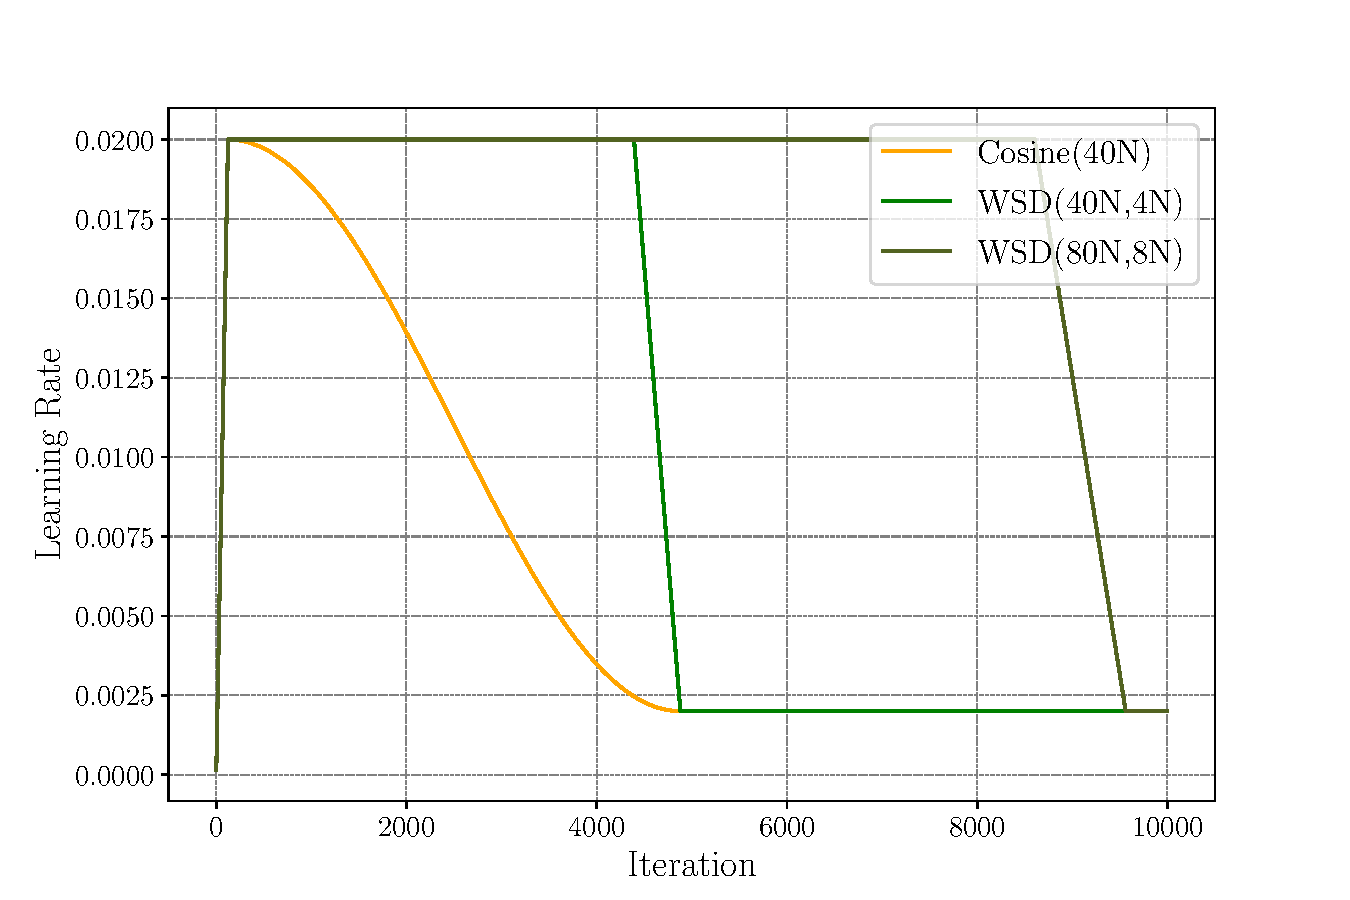
\includegraphics[width=0.98\linewidth]{Fig/lr.pdf}
        \caption{Illustrative comparison between Cosine LRS and WSD LRS. The WSD LRS with different end steps share the same stable training stage. }\label{fig:learning_rate_scheduler_diagram}
    \end{minipage}
        \begin{minipage}{0.45\linewidth}
    \centering
    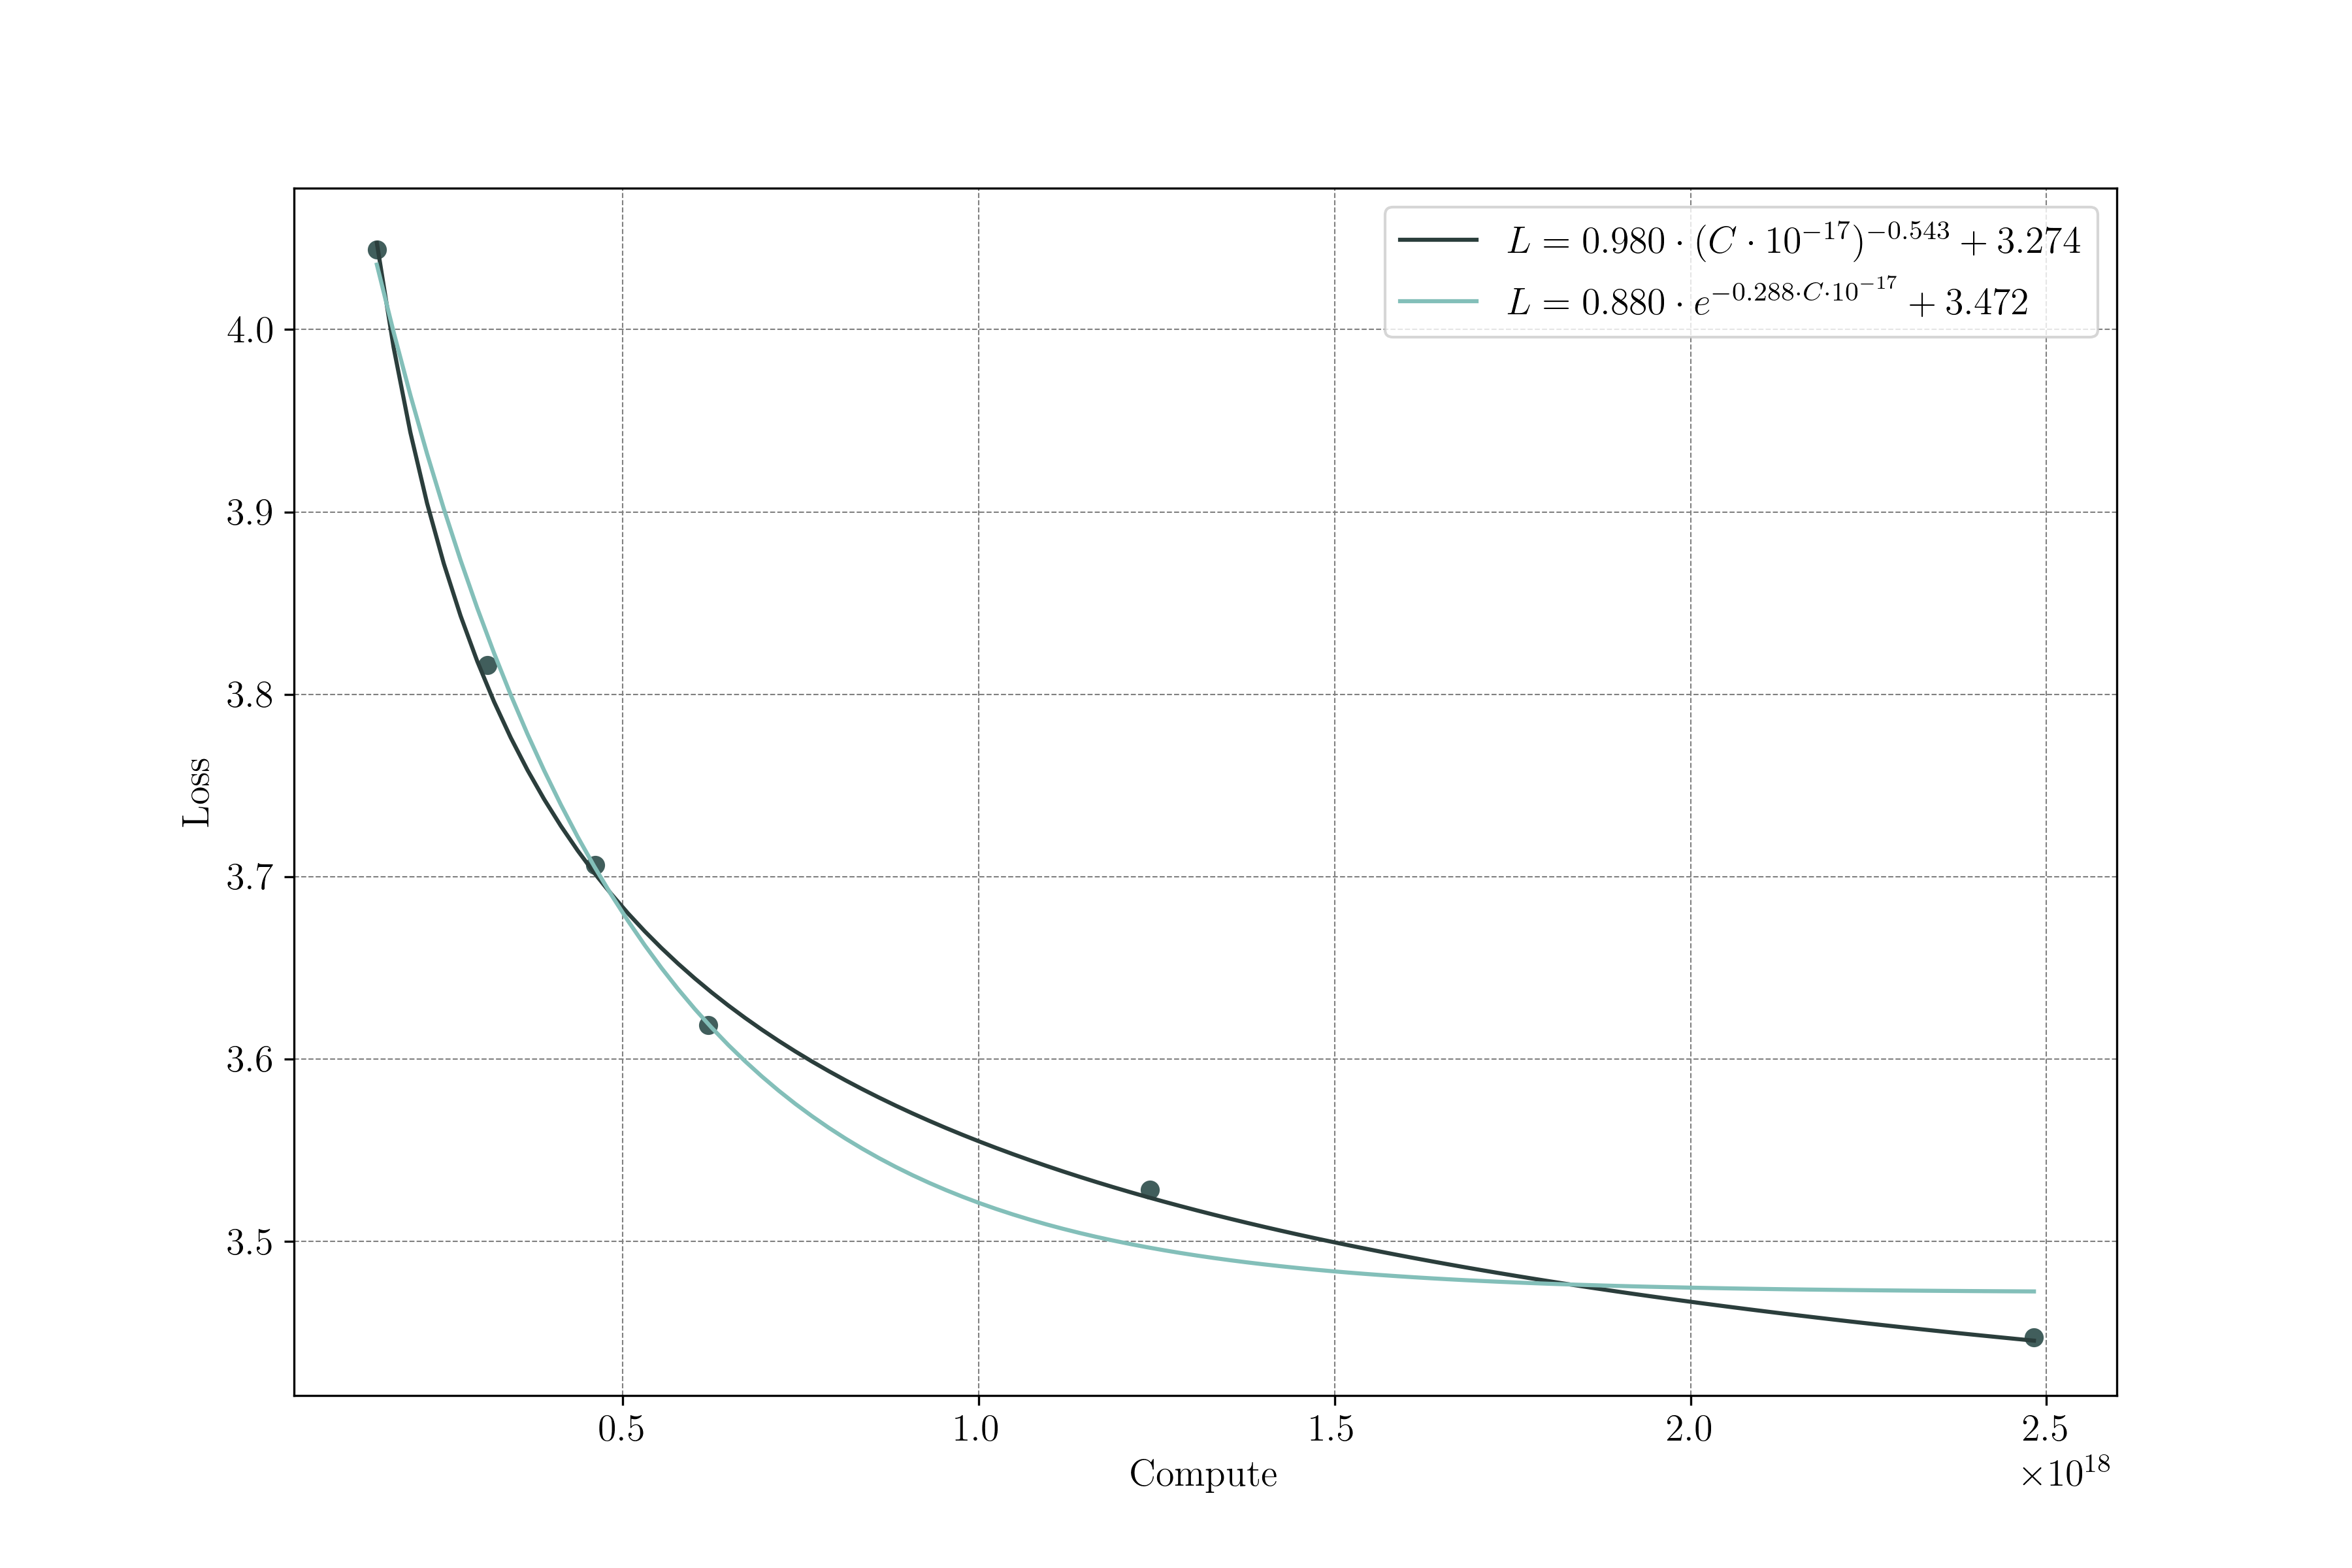
\includegraphics[width=1.05\linewidth]{Fig/fit_continuetrain.png}
    \caption{We use two different function forms to fit the data scaling law achieved by WSD LRS and choose power law as the best fit.}
    \label{fig:fit_continue_train}
    \end{minipage}
\end{figure}


\subsection{Fitting the Data Scaling Law}
\label{app:fittingdatascaling}
In this section, we describe the fitted data scaling law for continue training with WSD LRS. 
Each point in Figure~\ref{fig:fit_continue_train} is the end of the decay stage in WSD LRS with a different end step. We try two function forms: exponential and polynomial. The fitted result shows that the polynomial scaling law is still the best for continue training.
% \begin{figure}[!htbp]
%     \centering
%     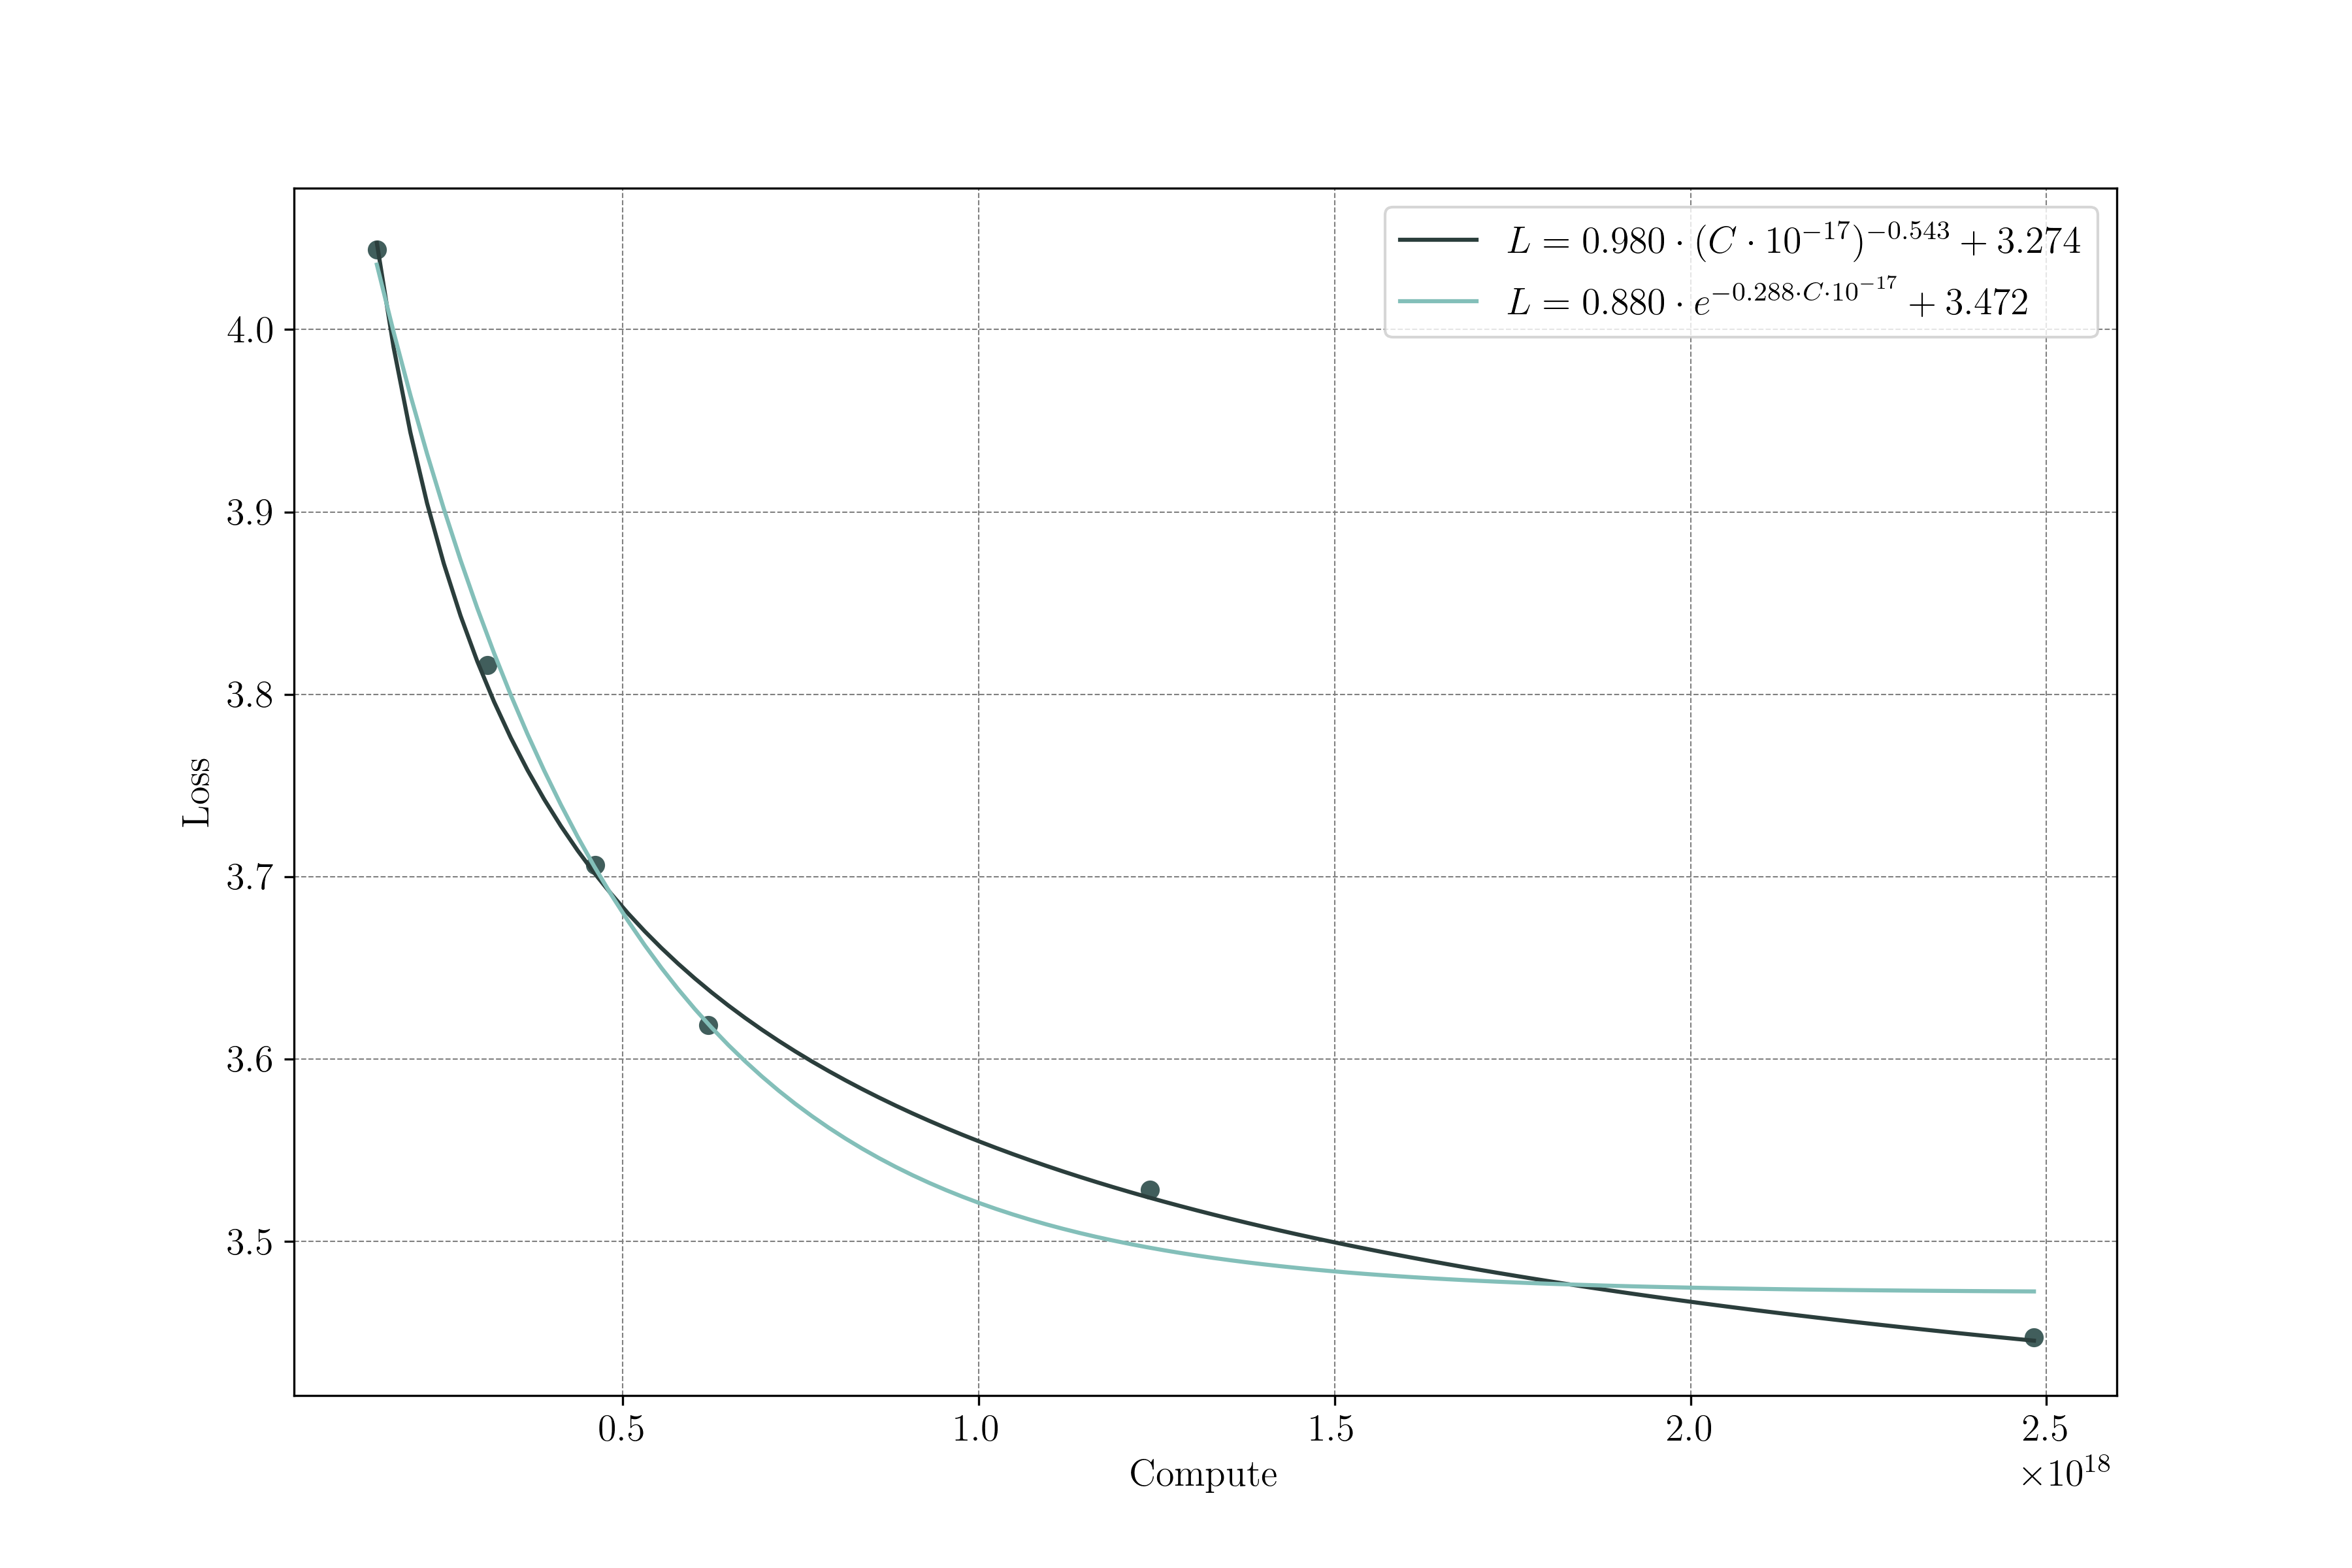
\includegraphics[width=0.7\linewidth]{Fig/fit_continuetrain.png}
%     \caption{We use two different function forms to fit the data scaling law achieved by WSD LRS and choose power law as the best fit.}
%     \label{fig:continue_train}
% \end{figure}

\subsection{Individual Figure for Model-Data Scaling Law}
For each task and model, the scaling law $L(N, D)$'s fitness with real loss values along the data axis is plotted in Figure~\ref{fig:individual_task_datascalinglaw}.

\subsection{Analysis of Llama2's Data-to-Model Ratio}
As mentioned in Section~\ref{scalinglawwsdlrs}, we analyze Llama2's Data-to-Model Ratio based on their training loss curve. The extracted loss is plotted on the left of Figure~\ref{fig:llamascaling}. We convert the x-axis to computation Flops to compare the computed optimal regime on the right part of the Figure. 

\begin{figure}
    \centering
    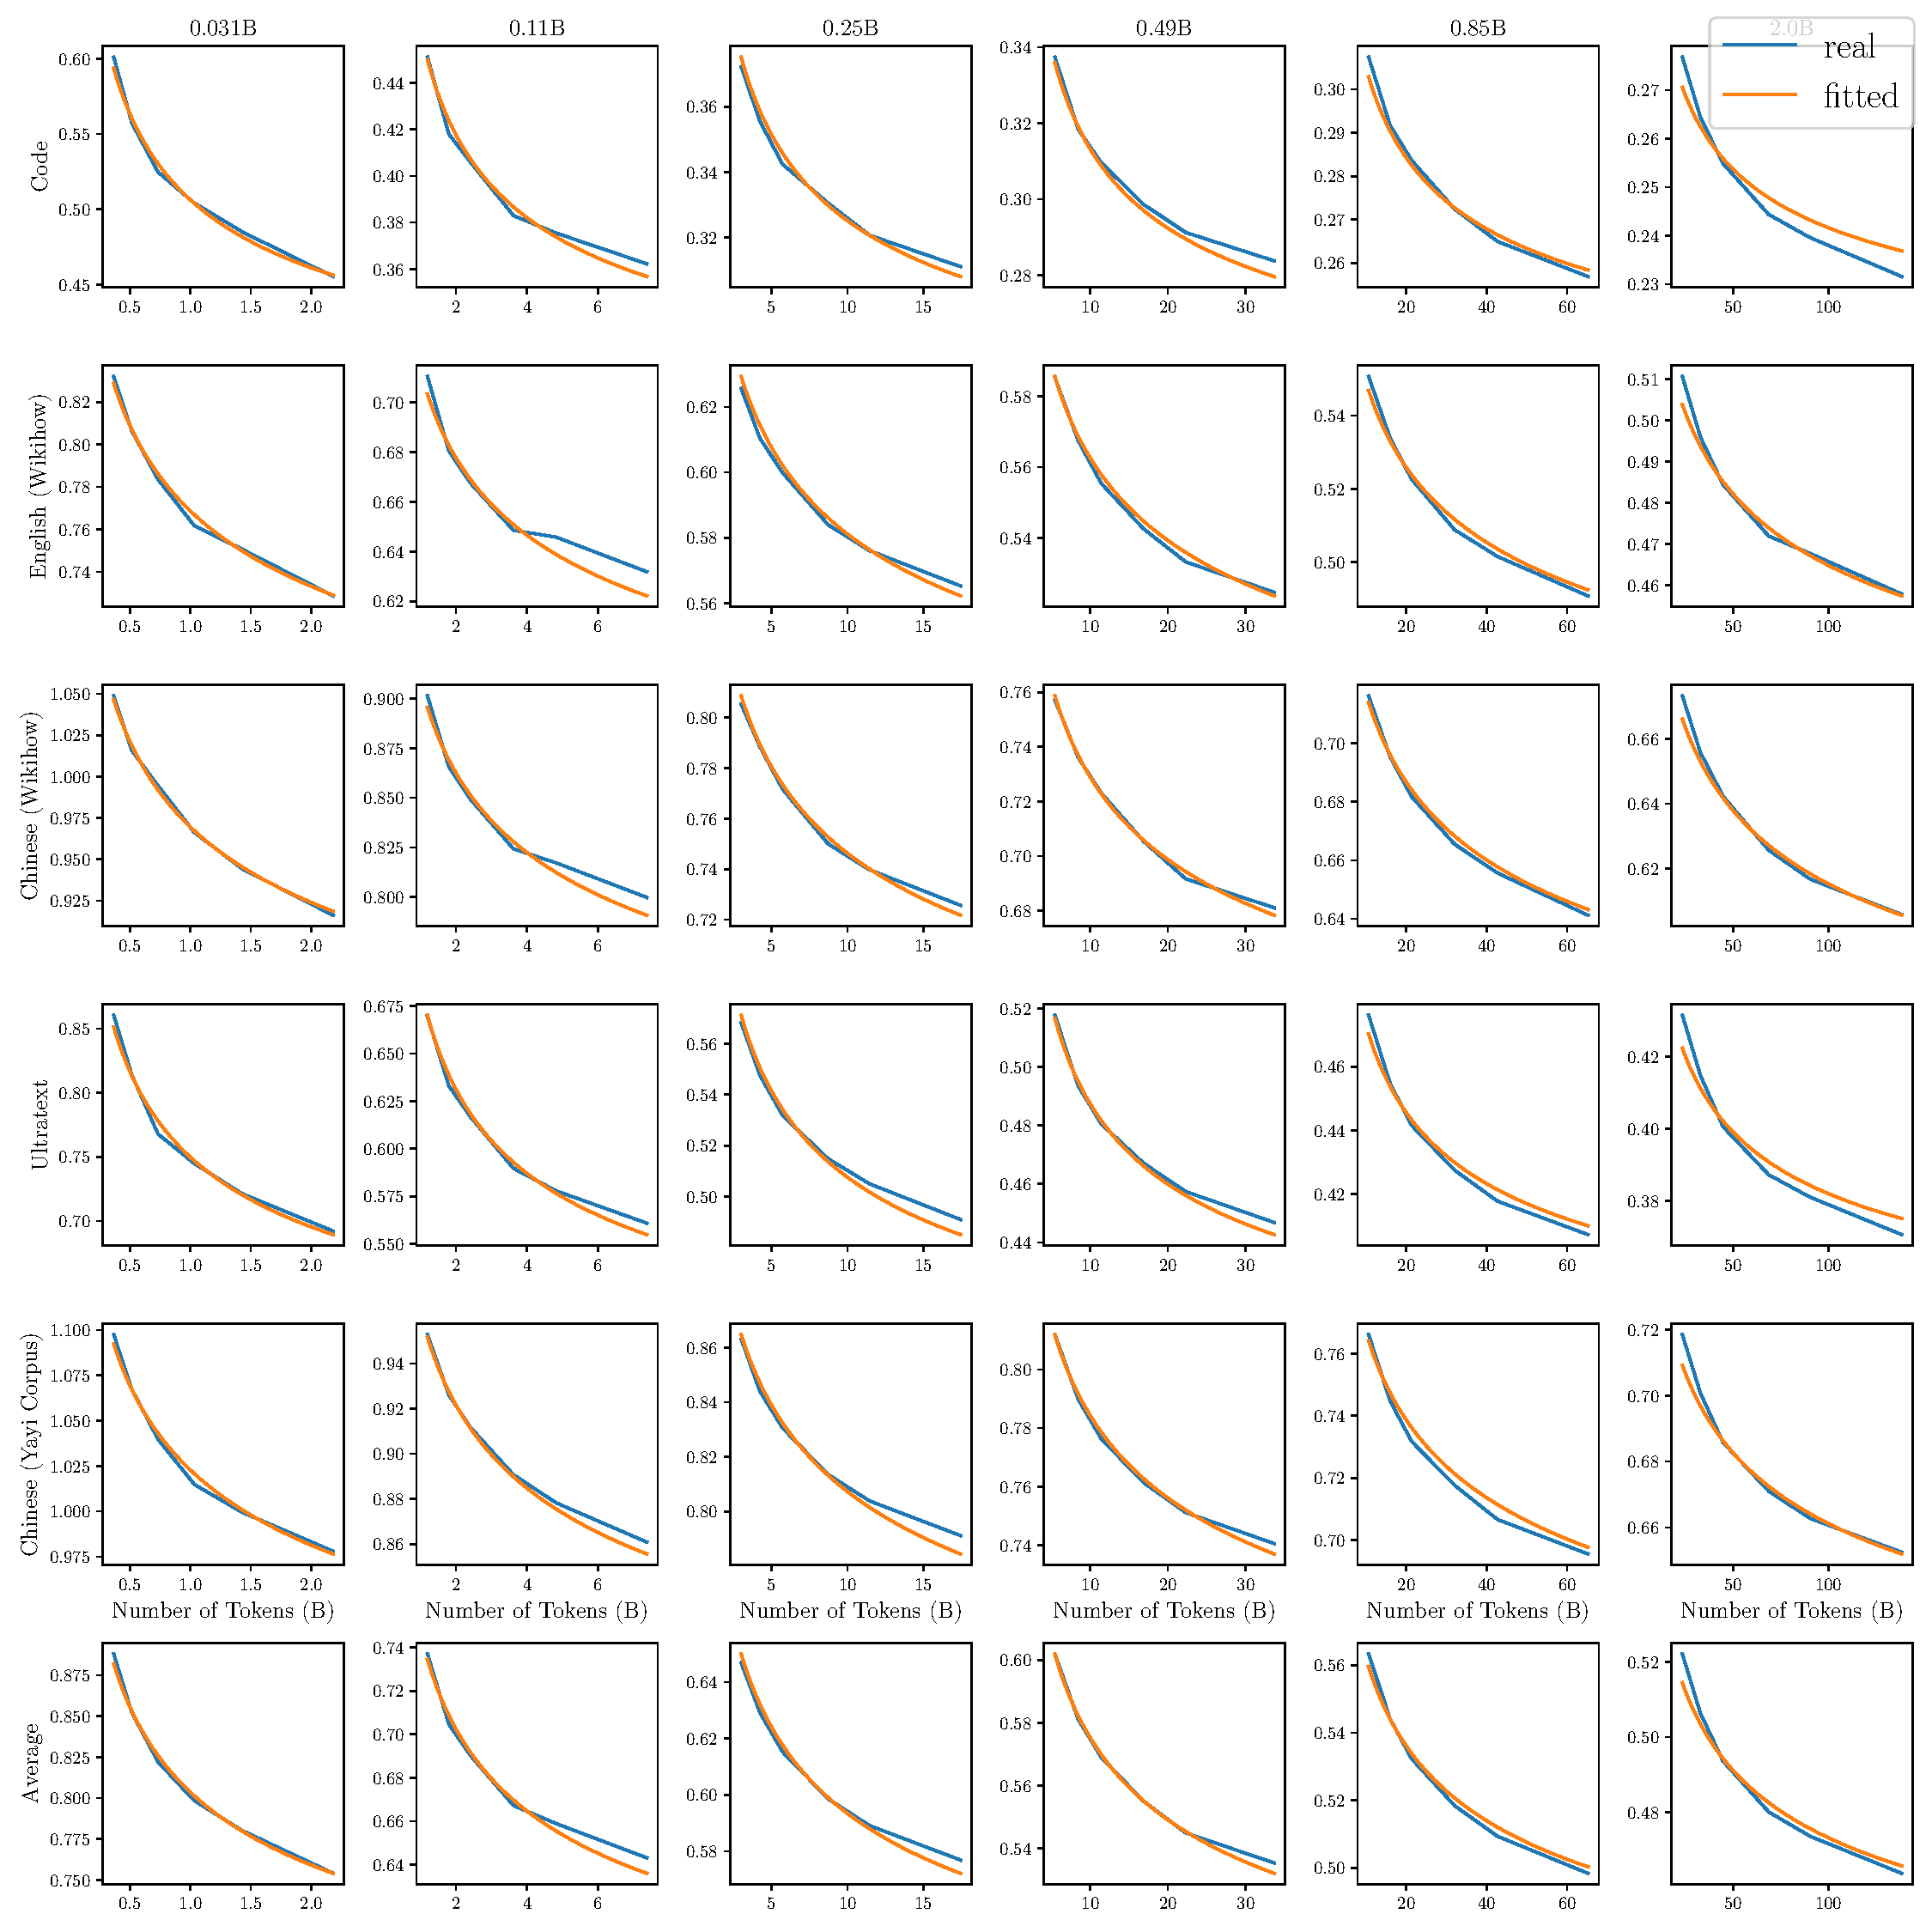
\includegraphics[width=1.0\textwidth]{Fig/individual_task_datascalinglaw.pdf}
    \caption{The fitted scaling law plotted along the data amount axis for each model and each task. The fitted result is satisfying except for the last checkpoints of the 0.11B and 0.25B model. }
    \label{fig:individual_task_datascalinglaw}
\end{figure}


\begin{figure}
    \centering
    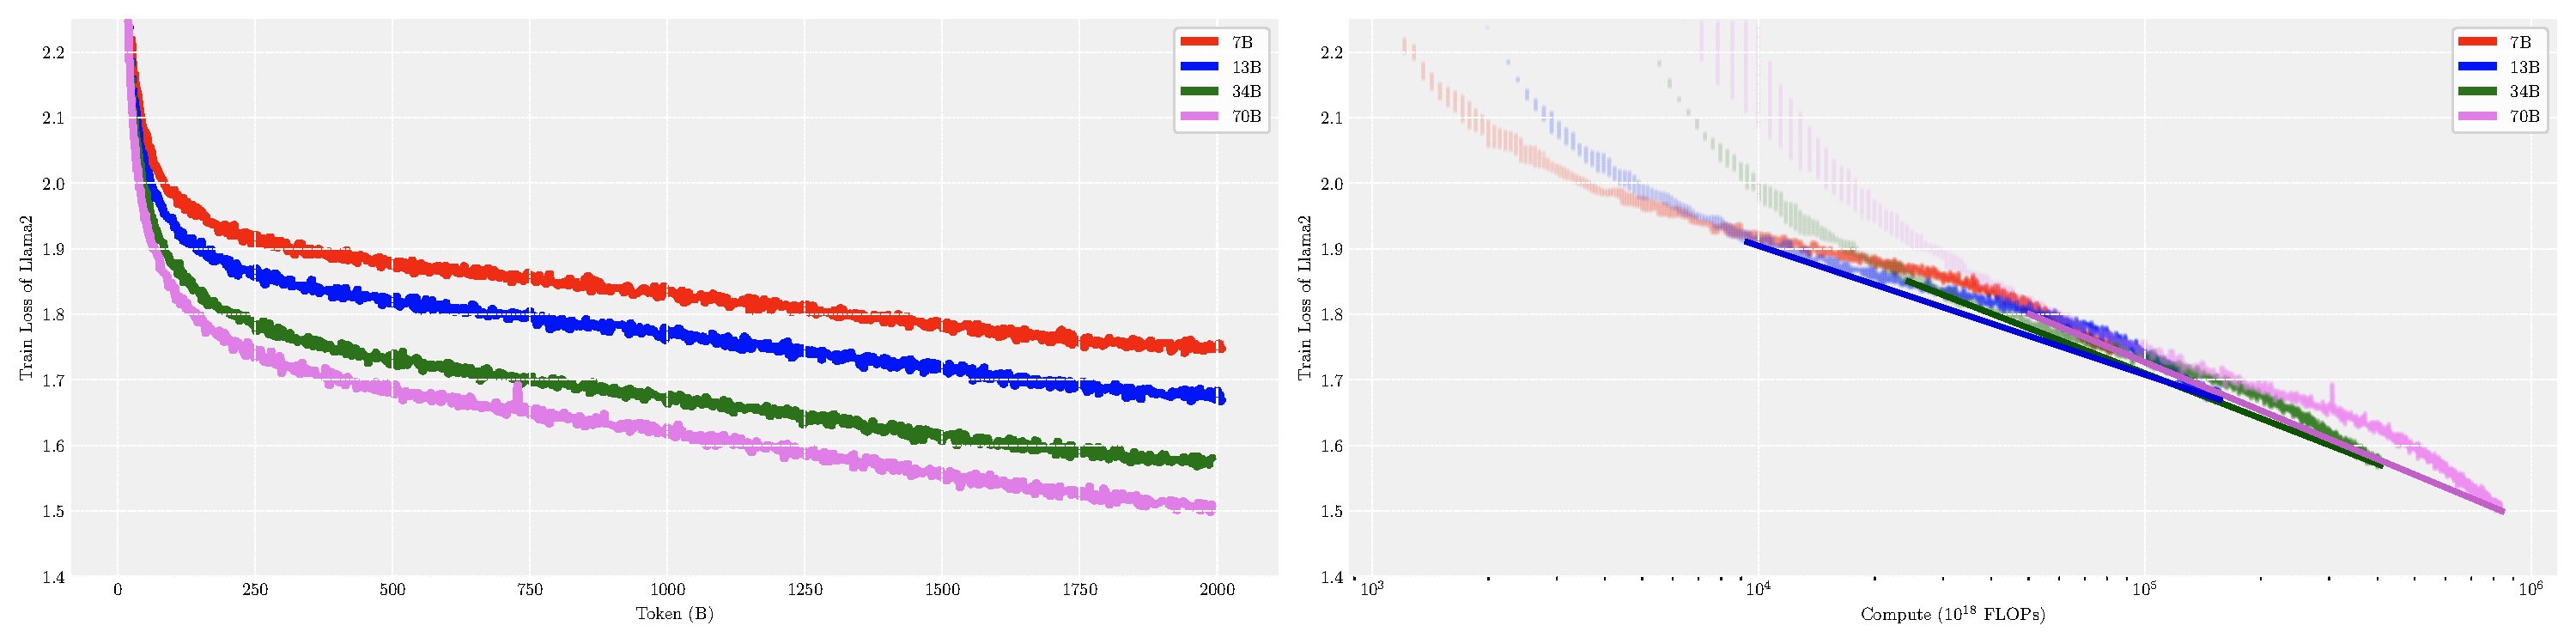
\includegraphics[width=1.0\textwidth]{Fig/llama2_scaling.pdf}
    \caption{We extract the training loss data from Llama2 paper (left part) and estimate the compute optimal $\frac{D_{opt}}{N_{opt}}$ in their paper using the right part. The straight lines are plotted to estimate the optimal loss envelope assuming using WSD Scheduler.}
    \label{fig:llamascaling}
\end{figure}



\section{MiniCPM's Vocabulary}
\label{app:tokenizer}

Despite being small in parameter size, MiniCPM targets modeling diverse data distribution, excelling in English and Chinese. Therefore, our vocabulary is relatively large. For the 2.4B model, we use a tokenizer consisting of 122,753 tokens (denoted by MiniCPMTokenizer-120K). This vocabulary is constructed from extensive and diverse language data, utilizing the sentencepiece library~\footnote{\url{https://github.com/google/sentencepiece}} for Byte Pair Encoding (BPE)~\citep{sennrich-etal-2016-neural}, and includes special symbols like traditional Chinese characters, rare characters, emojis, and special symbols such as Greek letters, Cyrillic letters, etc.

For the SLM, the embedding parameters will take up a lot of parameter space if the vocabulary is large. Therefore, for our 1.2B model, we use a smaller vocab MiniCPMTokenizer-70K. Compared to the MiniCPMTokenizer-120K tokenizer, we have re-trained the tokenization on the same documents, while setting the max number of vocabs to 64,000. For the special characters, we only add the traditional Chinese characters, emojis, and special symbols, but leave out the rare characters in Chinese. 

We conduct evaluations on 300,000 documents in Chinese, English, code, and academic papers that are not in the training set of the Tokenizer. The MiniCPM-120K tokenizer achieves the highest compression ratio (Bytes/Tokens).



\begin{table}[htbp]
\centering
\begin{tabular}{lccccc}
\toprule
  & {\textbf{Baichuan2}}  & {\textbf{ChatGLM2}} & {\textbf{Llama2}} & {\textbf{MiniCPM-120K}}  & {\textbf{MiniCPM-70K}}\\
\midrule
Vocab Size & 125,696 & 64,794 & 32,000 & 122,753 & 73,440\\
\midrule
\multicolumn{6}{c}{\textbf{Compression Rate} (Bytes/Tokens) }\\
\midrule
Chinese & 3.64   & 3.54  & 1.87  & \textbf{3.73} &  3.56 \\
English & 4.12   & 4.02  & 3.78  & \textbf{4.14} & 4.02 \\
Code    & 2.71   & 2.71  & 2.74  & \textbf{2.81} & 2.76 \\
Paper   & 2.74   & 2.88  & \textbf{2.97}  & 2.93 & 2.88\\
\midrule
Average & 3.30   & 3.29  & 2.84  & \textbf{3.40}  & 3.31 \\
\bottomrule
\end{tabular}
\caption{Compression ratio comparison.}
\label{tab:compression_ratio}
\end{table}

